\begin{frame}{Addestramento sostenibile - Introduzione}
    \begin{wrapfigure}{r}{0.6\textwidth}
        \centering
        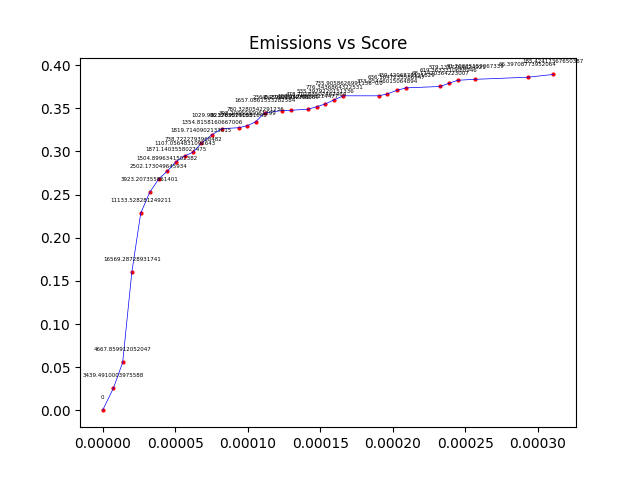
\includegraphics[width=0.6\textwidth]{images/curve_emissions_score.png}
        \caption{Andamento score e emissioni}
    \end{wrapfigure} 
Approssimazione della derivata della curva:
\begin{equation*}
    \frac{f(x_{i+1}) - f(x_i)}{x_{i+1} - x_i}
\end{equation*}
\end{frame}

\begin{frame}{Addestramento sostenibile - Esplorazione}
    \begin{itemize}
        \item \textbf{Scopo}: capire se è possibile addestrare un modello di raccomandazione in modo sostenibile
        \item \textbf{Esperimento 1:} MovieLens1M con soglia 50 e 5 epoche
        \item \textbf{Esperimento 2:} LastFM con soglia 30 e 7 epoche
        \item \textbf{Esperimento 3:} Amazon\_Books con soglia 40 e 6 epoche
        \item \textbf{Conclusioni:} Alcuni modelli (es. DGCF) sono molto sensibili al nuovo criterio, altri (es. DMF) meno
    \end{itemize}
\end{frame}

\begin{frame}{Addestramento sostenibile - Esempi di risultati}
    \begin{table}[H]
        \centering
        \setlength\tabcolsep{20pt} % Aumenta lo spazio tra le colonne
        \setlength{\arrayrulewidth}{0.5pt}
        \begin{tabularx}{\textwidth}{X X}
            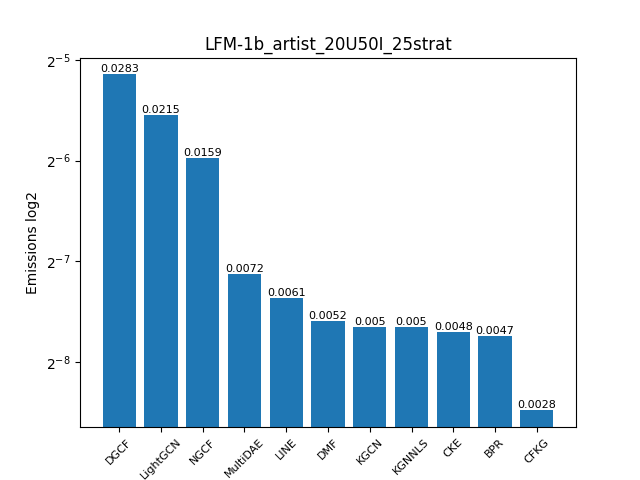
\includegraphics[width=0.35\textwidth, height=0.35\textheight, trim=0 0 0 0]{images/emissions_LFM-1b_artist_20U50I_25strat_earlyClassic.png} &
            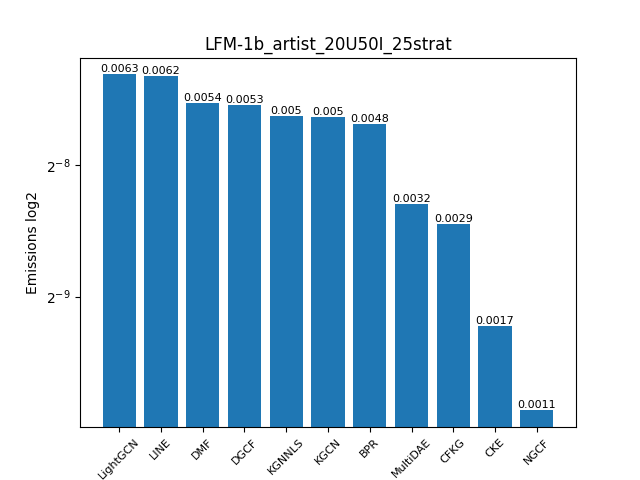
\includegraphics[width=0.35\textwidth, height=0.35\textheight, trim=0 0 0 0]{images/emissions_LFM-1b_artist_20U50I_25strat_earlyModified.png} \\
            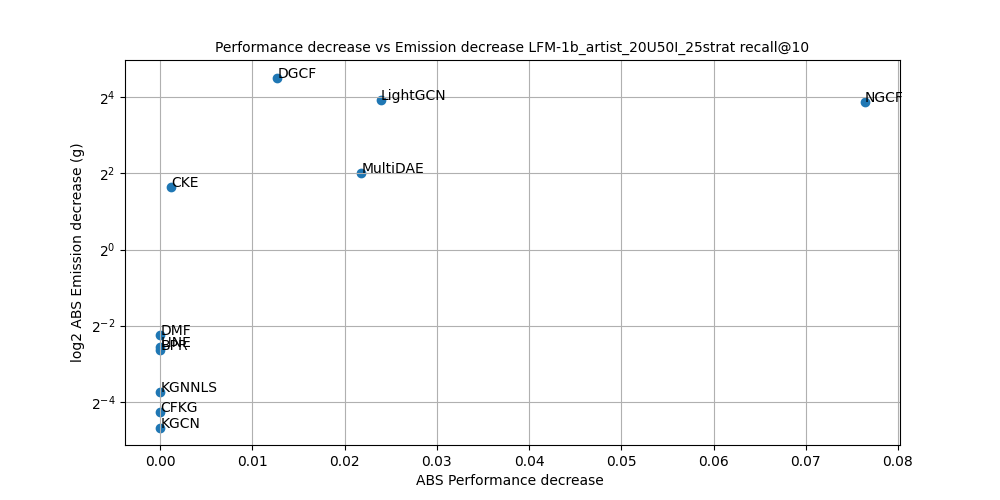
\includegraphics[width=0.35\textwidth, height=0.35\textheight, trim=0 0 0 0]{images/decrement_recall@10_LFM-1b_artist_20U50I_25strat.png} &
            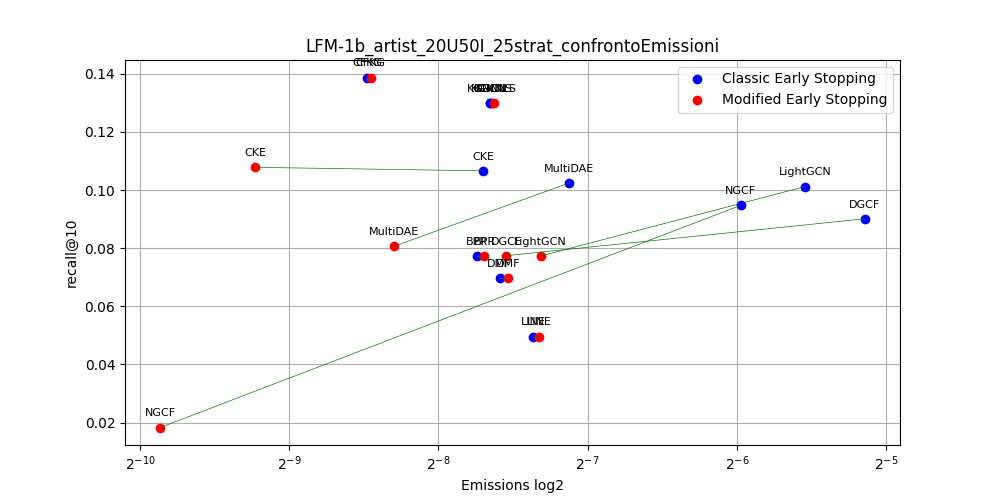
\includegraphics[width=0.35\textwidth, height=0.35\textheight, trim=0 0 0 0]{images/recall@10_LFM-1b_artist_20U50I_25strat_comparison.png} \\
        \end{tabularx}
        \caption{Esempi di risultati}
    \end{table}
\end{frame}


\begin{frame}{Addestramento sostenibile - Confronto criteri}
    \begin{itemize}
        \item \textbf{Scopo}: confrontare i criteri di addestramento sostenibile (dataset MovieLens1M)
        \item \textbf{Esperimento 1:} Soglia 40, 5 epoche
        \item \textbf{Esperimento 2:} Soglia 30, 5 epoche
        \item \textbf{Esperimento 3:} Soglia 40, 6 epoche
        \item \textbf{Esperimento 4:} Soglia 30, 6 epoche
        \item \textbf{Esperimento 5:} Soglia 40, 7 epoche
        \item \textbf{Esperimento 6:} Soglia 30, 7 epoche
\end{itemize}
\end{frame}

\begin{frame}{Addestramento sostenibile - Esempio sensibilità}
    \begin{figure}[H]
        \centering
        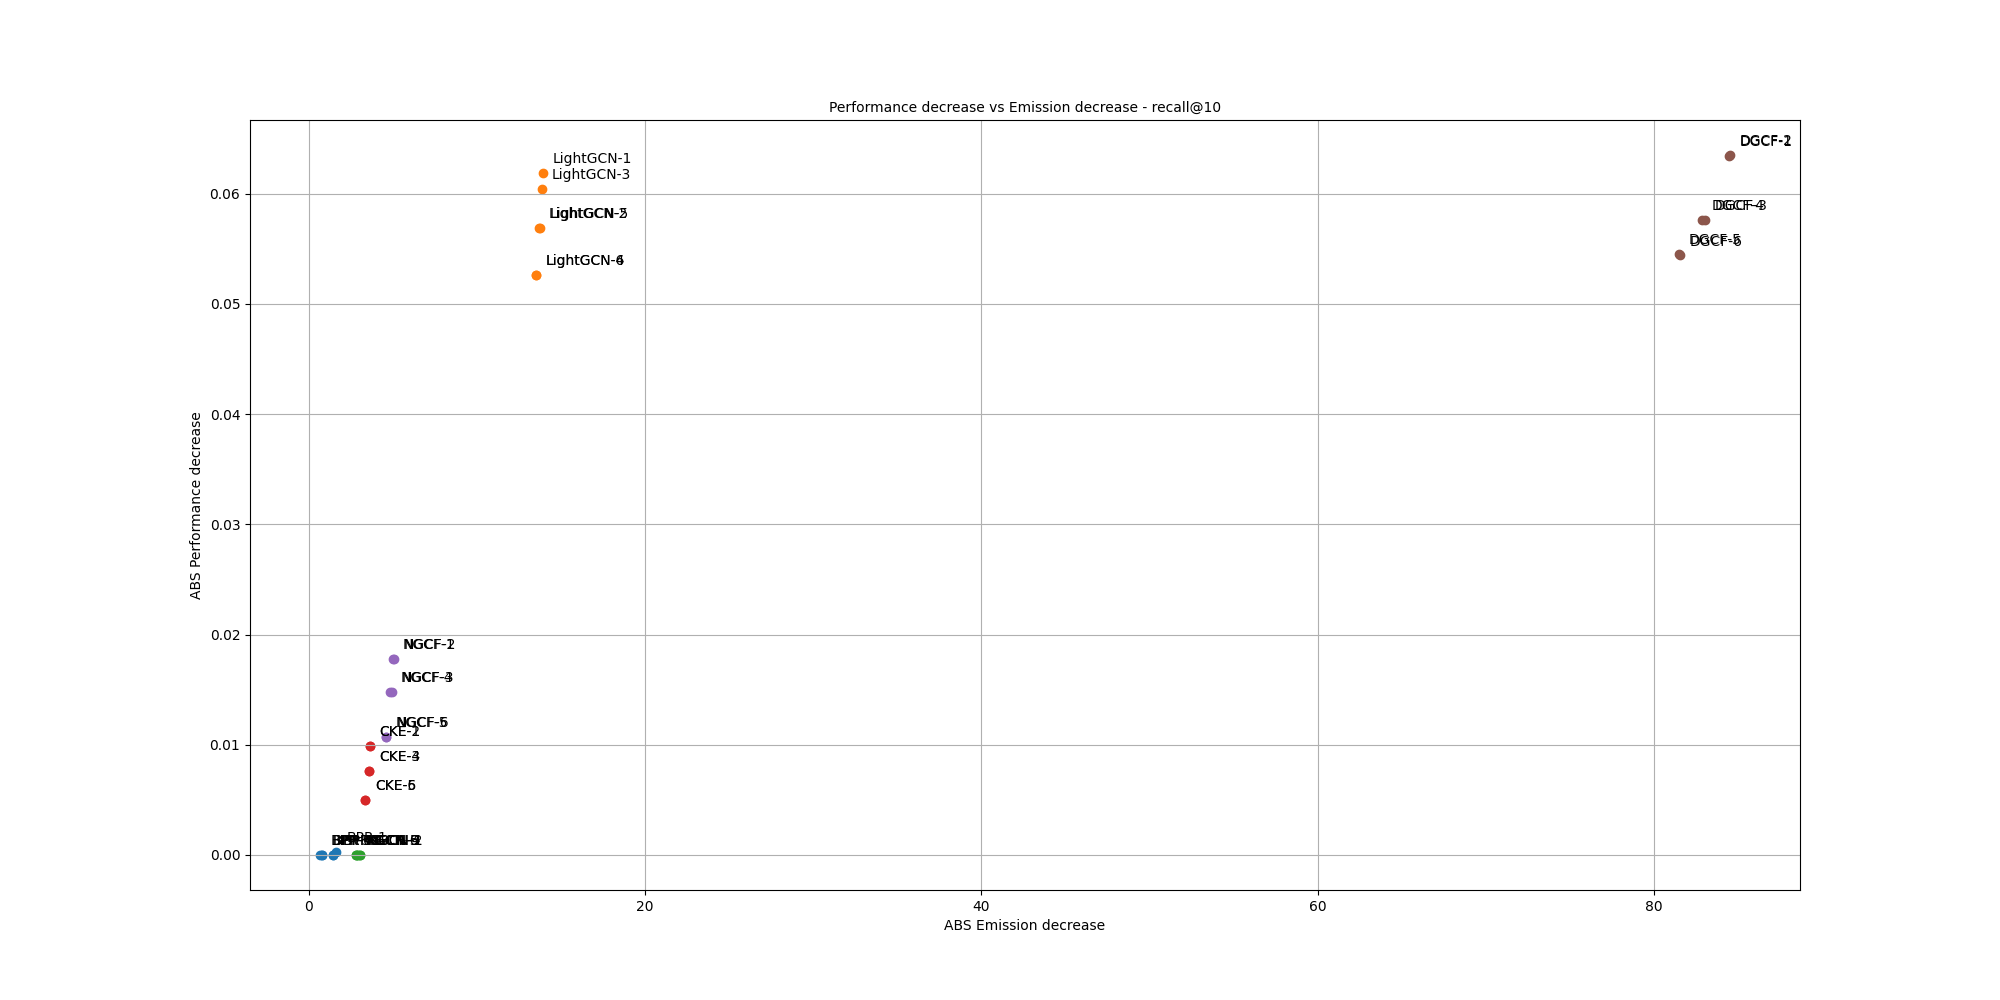
\includegraphics[width=0.8\textwidth]{images/sensibility_recall@10.png}
        \caption{Sensibilità dei parametri con metrica Recall@10}
    \end{figure}
\end{frame}


\begin{frame}{Addestramento sostenibile - Risultati confronto criteri}
\tiny
\begin{table}[H]
    \centering
    \begin{tabular}{|c|c|c|}
        \hline
        \textbf{Modello} & \textbf{Parametro più impattante} & \textbf{Migliori risultati} \\
        \hline
        BPR & Soglia & Soglia 40 e 6 epoche \\
        \hline
        CFKG & Soglia & Soglia 40 e 6 epoche \\
        \hline
        CKE & Epoche consecutive & Soglia 40 e 6 epoche \\
        \hline
        DMF & Nessuno predominante & Soglia 40 e 7 epoche \\
        \hline
        KGCN & Epoche consecutive & Soglia 40 e 5 epoche \\
        \hline
        KGNNLS & Soglia & Soglia 40 e 5 epoche \\
        \hline
        LINE & Soglia & Soglia 40 e 7 epoche \\
        \hline
        MultiDAE & Soglia & Soglia 40 e 7 epoche \\
        \hline
        LightGCN & Soglia & Soglia 40 e 6 epoche \\
        \hline
        NGCF & Epoche consecutive & Soglia 40 e 5 epoche \\
        \hline
        DGCF & Epoche consecutive & Soglia 40 e 6 epoche \\
        \hline
    \end{tabular}
    \caption{Parametri più impattanti e migliori risultati per ciascun modello}
\end{table}

\tiny
\begin{table}[H]
    \centering
        \begin{tabular}{|c|c|c|c|}
            \hline
            \textbf{Tipo di Modello} & \textbf{Parametro predominante} & \textbf{Numero di Modelli} & \textbf{Modelli} \\ \hline
            Collaborative Filtering & Soglia & 5 & BPR, DMF, LightGCN, MultiDAE, LINE \\ \hline
            Collaborative Filtering & Epoche & 2 & NGCF, DGCF \\ \hline
            Knowledge Aware & Soglia & 2 & CFKG, KGNNLS \\ \hline
            Knowledge Aware & Epoche & 2 & CKE, KGCN \\ \hline
        \end{tabular}
    \caption{Riassunto dei parametri dominanti per tipo di modello}
\end{table}

\end{frame}